%
% @author   Christopher Schmitt & Matthew Warren
% @version  3/29/2020
% @license  MIT
%


\documentclass{article}


%
% Document Imports
%

\usepackage{fancyhdr}
\usepackage{extramarks}
\usepackage{amsmath}
\usepackage{amssymb}
\usepackage{amsthm}
\usepackage{amsfonts}
\usepackage{color}
\usepackage{listings}
\usepackage[color]{register}
\usepackage{booktabs}



%
% Document Configuration
%

\newcommand{\hwAuthor}{Christopher K. Schmitt and Matthew Warren}
\newcommand{\hwSubject}{CS 358}
\newcommand{\hwSection}{Section 01}
\newcommand{\hwSemester}{Spring 2020}
\newcommand{\hwAssignment}{Progress Report 2}

\definecolor{dkgreen}{rgb}{0,0.6,0}
\definecolor{gray}{rgb}{0.5,0.5,0.5}
\definecolor{mauve}{rgb}{0.58,0,0.82}

\lstset{
  frame=tb,
  language=Verilog,
  aboveskip=3mm,
  belowskip=3mm,
  showstringspaces=false,
  columns=flexible,
  basicstyle=\ttfamily,
  numbers=none,
  numberstyle=\tiny\color{gray},
  keywordstyle=\color{blue},
  commentstyle=\color{dkgreen},
  stringstyle=\color{mauve},
  breaklines=true,
  breakatwhitespace=true,
  tabsize=3
}


%
% Document Environments
%

\setlength{\headheight}{65pt}
\pagestyle{fancy}
\lhead{\hwAuthor}
\rhead{
  \hwSubject \\
  \hwSection \\
  \hwSemester \\
  \hwAssignment
}

\newenvironment{problem}[1]{
  \nobreak\section*{#1}
}{}


%
% Document Start
%

\begin{document}
  \begin{problem}{Instruction Set Architecture}
    \paragraph{}
    We fully implement a simplified single-cycle MIPS architecture, including 
    branch, store, and load instructions.

    \begin{table}[]
      \begin{tabular}{@{}lllp{6.8cm}@{}}
        \toprule
        Instruction & Opcode & Format & Description \\ \midrule
        add & 0000 & R-Type & Adds \$rs and \$rt together using arithmetic addition, places the sum in \$rt \\
        sub & 0001 & R-Type & Subtract \$rt from \$rs, places the difference in \$rt \\
        and & 0010 & R-Type & Perform bitwise ANDing on \$rs and \$rt, place the result in \$rd \\
        or & 0011 & R-Type & Perform bitwise ORing on \$rs and \$rt, place the result in \$rd \\
        addi & 0100 & I-Type & Add \$rs to immediate value, place the result in \$rt \\
        lw & 0101 & I-Type & Load the value at \$rs + VALUE into \$rt \\
        sw & 0110 & I-Type & Store \$rt at \$rs + VALUE \\
        slt & 0111 & R-Trpe & Put 0x01 in \$rd if \$rs $<$ \$rt, 0x00 otherwise \\
        beq & 1000 & I-Type & Set PC to PC + VALUE if \$rs $=$ \$rt, PC + 0x01 otherwise \\
        bne & 1001 & I-Type & Set PC to PC + VALUE if \$rs $\ne$ \$rt, PC + 0x01 otherwise \\ \bottomrule
      \end{tabular}
    \end{table}
    
    \begin{register}{H}{R-Type}{}
      \begin{center}
        \regfield[green!30]{}{4}{12}{{op}}
        \regfield[red!30]{}{2}{10}{{rs}}
        \regfield[blue!30]{}{2}{8}{{rt}}
        \regfield[orange!30]{}{2}{6}{{rd}}
        \regfield[gray!30]{}{6}{0}{{unused}}
      \end{center}
    \end{register}

    \begin{register}{H}{I-Type}{}
      \begin{center}
        \regfield[green!30]{}{4}{12}{{op}}
        \regfield[red!30]{}{2}{10}{{rs}}
        \regfield[blue!30]{}{2}{8}{{rt}}
        \regfield[orange!30]{}{8}{0}{{value}}
      \end{center}
    \end{register}

    In the above diagrams, \emph{op} is the opcode, \emph{rs} is the
    source register, \emph{rt} is the target/destination register, and
    \emph{rd} is the destination register.  Value is the immediate value
    in I-Type instructions.
  \end{problem}

  \begin{problem}{Control Table}
    \begin{table}[]
      \begin{tabular}{@{}llllllll@{}}
      Operation & RegDst & ALUSrc & MemToReg & RegWrite & MemWrite & Branch & ALUOp \\ \midrule
      add & 1 & 0 & 0 & 1 & 0 & 0 & 00 \\
      sub & 1 & 0 & 0 & 1 & 0 & 0 & 01 \\
      and & 1 & 0 & 0 & 1 & 0 & 0 & 10 \\
      or & 1 & 0 & 0 & 1 & 0 & 0 & 10 \\
      addi & 0 & 1 & 0 & 1 & 0 & 0 & 00 \\
      lw & 0 & 1 & 1 & 1 & 0 & 0 & 00 \\
      sw & 0 & 0 & 0 & 0 & 1 & 0 & 00 \\
      slt & 1 & 0 & 0 & 1 & 0 & 0 & 10 \\
      beq & 0 & 0 & 0 & 0 & 0 & 1 & 01 \\
      bne & 0 & 0 & 0 & 0 & 0 & 1 & 01
      \end{tabular}
    \end{table}
  \end{problem}

  \begin{problem}{Source Code}
    \lstinputlisting[language=Verilog, basicstyle=\scriptsize\ttfamily]{../processor.vl}
  \end{problem}

  \begin{problem}{Machine Translation}
    \lstinputlisting[basicstyle=\ttfamily]{../testSwap.txt}
  \end{problem}

  \begin{problem}{Output (No Branch)}
    \begin{center}
      \begin{lstlisting}[basicstyle=\footnotesize\ttfamily]
clk         pc  instruction             data
1           0   0101000100000000        0000000000000111
0           1   0101001000000001        0000000000000101
1           1   0101001000000001        0000000000000101
0           2   0111011011000000        0000000000000000
1           2   0111011011000000        0000000000000000
0           3   1001110000000010        0000000000000000
1           3   1001110000000010        0000000000000000
0           4   0110000100000001        0000000000000001
1           4   0110000100000001        0000000000000001
0           5   0110001000000000        0000000000000000
1           5   0110001000000000        0000000000000000
0           6   0101000100000000        0000000000000111
1           6   0101000100000000        0000000000000111
0           7   0101001000000001        0000000000000101
1           7   0101001000000001        0000000000000101
0           8   0001011001000000        0000000000000010
1           8   0001011001000000        0000000000000010
      \end{lstlisting}
    \end{center}
  \end{problem}

  \begin{problem}{Output (Branch)}
    \begin{center}
      \begin{lstlisting}[basicstyle=\footnotesize\ttfamily]
clk         pc  instruction             data
1           0   0101000100000000        0000000000000101
0           1   0101001000000001        0000000000000111
1           1   0101001000000001        0000000000000111
0           2   0111011011000000        0000000000000001
1           2   0111011011000000        0000000000000001
0           3   1001110000000010        0000000000000001
1           3   1001110000000010        0000000000000001
0           5   0110001000000000        0000000000000000
1           5   0110001000000000        0000000000000000
0           6   0101000100000000        0000000000000101
1           6   0101000100000000        0000000000000101
0           7   0101001000000001        0000000000000111
1           7   0101001000000001        0000000000000111
0           8   0001011001000000        1111111111111110
1           8   0001011001000000        1111111111111110
0           9   xxxxxxxxxxxxxxxx        xxxxxxxxxxxxxxxx
1           9   xxxxxxxxxxxxxxxx        xxxxxxxxxxxxxxxx
      \end{lstlisting}
    \end{center}
  \end{problem}

  \pagebreak
  \begin{problem}{CPU Complete Diagram}
    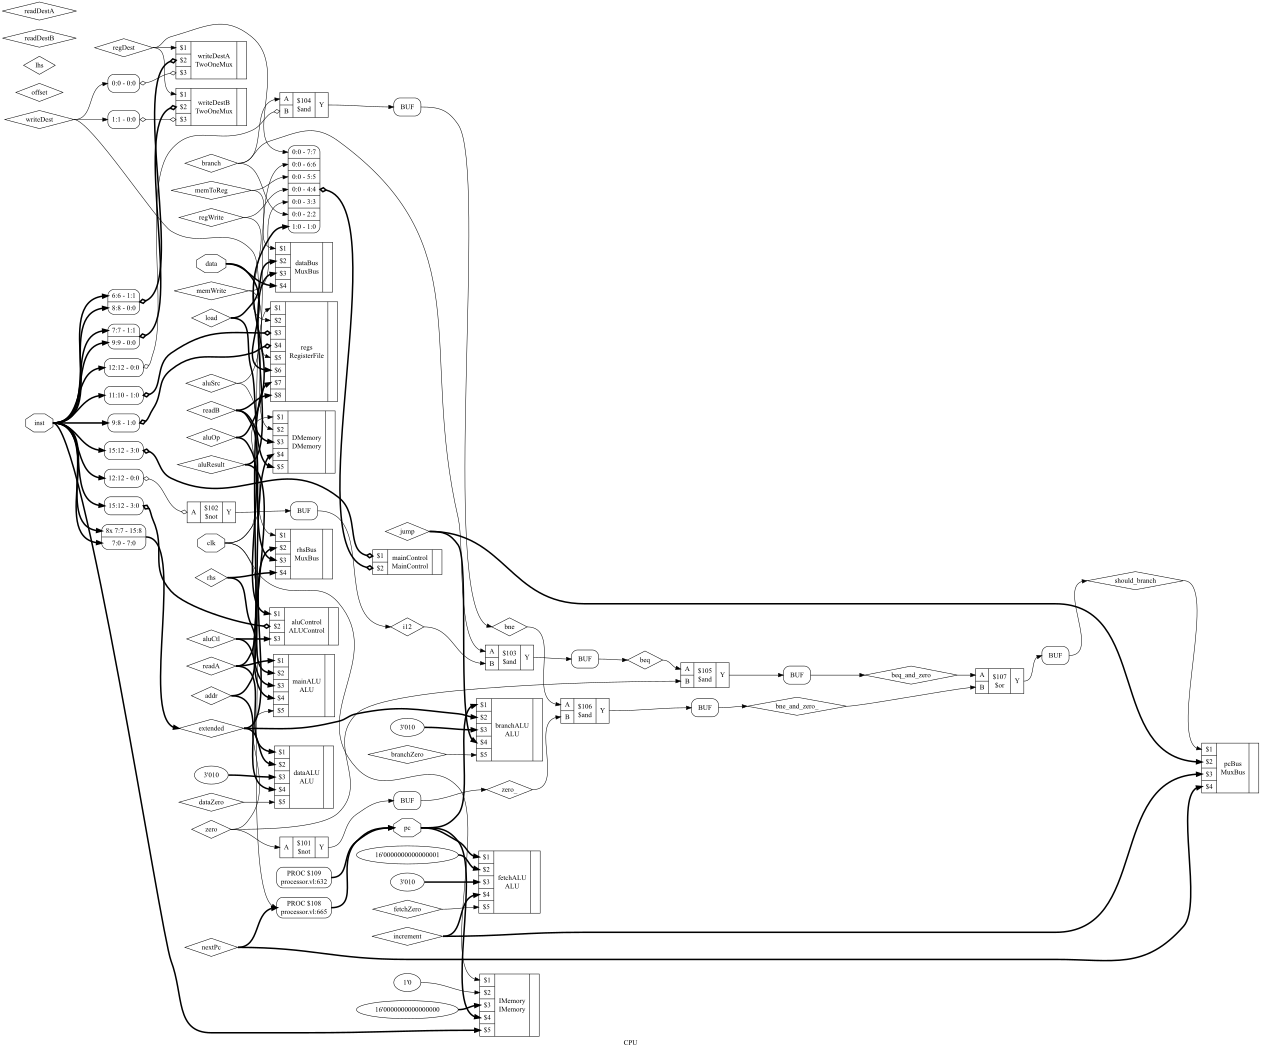
\includegraphics[scale=0.15]{../images/bitmap.png}
  \end{problem}
\end{document}